\documentclass[preprint]{article}
%\renewcommand{\rmdefault}{ppl}
%\usepackage{personal}
\usepackage{graphicx}
\usepackage{placeins}

\usepackage{amsmath}
\usepackage{wasysym}
\usepackage{amssymb}

\usepackage{array}
\newcolumntype{L}[1]{>{\raggedright\let\newline\\\arraybackslash\hspace{0pt}}m{#1}}
\newcolumntype{C}[1]{>{\centering\let\newline\\\arraybackslash\hspace{0pt}}m{#1}}
\newcolumntype{R}[1]{>{\raggedleft\let\newline\\\arraybackslash\hspace{0pt}}m{#1}}
\usepackage{booktabs}
\usepackage{tabularx}
%\usepackage[font=small]{caption}
%\usepackage[strings]{underscore}
%\usepackage{subfigure}
\usepackage{color}
\usepackage{floatflt}
\usepackage[table]{xcolor}
\definecolor{Gray}{gray}{0.9}
%\usepackage[boxed]{algorithm2e}
%\usepackage{lmacro}
%\topmargin=-0.5in\usepackage[table]{xcolor}
\definecolor{White}{rgb}{1,1,1}
\definecolor{Gray}{gray}{0.9}
\definecolor{LightCyan}{rgb}{0.88,1,1}
\usepackage{soul}
\usepackage{sidecap}
\graphicspath{{./Figures/}}
%\usepackage[margin=1.2in]{geometry}
\usepackage{hyperref}
\hypersetup{colorlinks=true,
citecolor=blue,
linkcolor=black,
urlcolor=black}

\usepackage{algorithm,algorithmicx}
\usepackage[noend]{algpseudocode}
\newcommand*\DNA{\textsc{dna}}

\newcommand*\Let[2]{\State #1 $\gets$ #2}
\algrenewcommand\algorithmicrequire{\textbf{Precondition:}}
\algrenewcommand\algorithmicensure{\textbf{Postcondition:}}
%\usepackage{fontspec}
%\setmainfont{Hoefler Text}
%\newcommand*\DNA{\textsc{dna}}
%
%\newcommand*\Let[2]{\State #1 $\gets$ #2}
%\algrenewcommand\alglinenumber[1]{
%    {\sf\footnotesize\addfontfeatures{Colour=888888,Numbers=Monospaced}#1}}
%\algrenewcommand\algorithmicrequire{\textbf{Precondition:}}
%\algrenewcommand\algorithmicensure{\textbf{Postcondition:}}

\title{{\bf \huge $\epsilon$}-Lexicase selection: a probabilistic and multi-objective analysis of lexicase selection in continuous domains}
%\author{William La Cava, Lee Spector, Jason Moore}




\begin{document}

%\numberofauthors{3}
%
%\alignauthor
%William La Cava\titlenote{corresponding author} \\
%       \affaddr{Department of Mechanical and Industrial Engineering}\\
%       \affaddr{University of Massachusetts}\\
%       \affaddr{Amherst, MA 01003}\\
%       \email{wlacava@umass.edu}
%%%\alignauthor
%%%Thomas Helmuth\\
%%%       \affaddr{Department of Computer Science}\\
%%%       \affaddr{University of Massachusetts}\\
%%%       \affaddr{Amherst, MA 01003}\\
%%%       \email{thelmuth@umass.edu}
%\alignauthor
%Lee Spector\\
%       \affaddr{School of Cognitive Science}\\
%       \affaddr{Hampshire College}\\
%       \affaddr{Amherst, MA 01002}\\
%       \email{lspector@hampshire.edu}
%\and
%\alignauthor
%Kourosh Danai\\
%       \affaddr{Department of Mechanical and Industrial Engineering}\\
%       \affaddr{University of Massachusetts}\\
%       \affaddr{Amherst, MA 01003}\\
%       \email{danai@engin.umass.edu}
%}

%\maketitle
%\ead{danai@ecs.umass.edu}
%\cortext[cor1]{Corresponding author}
%\address[mie]{D, , Amherst, MA 01003}
%\address[hc]{School of Cognitive Science, Hampshire College, Amherst MA 01002}
%

\maketitle
\begin{abstract}
Lexicase selection is a parent selection method that considers test cases separately, rather than in aggregate, when performing parent selection. As opposed to previous work that has demonstrated the ability of lexicase selection to solve difficult problems, the goal of this paper is to develop the theoretical underpinnings that explain its performance. To this end, we derive an analytical formula that gives the expected probabilities of selection under lexicase selection, given a population and its behavior. In addition, we expand upon the relation of lexicase selection to many-objective optimization methods to show the effect of lexicase, which is to select individuals on the boundaries of Pareto fronts in high-dimensional space. We show analytically why lexicase selection performs more poorly for certain sizes of population and training cases, and why it has been shown to perform more poorly in continuous error spaces. To addres this last concern, we introduce $\epsilon$-lexicase selection, which modifies the pass condition defined in lexicase selection to allow near-elite individuals to pass cases, thereby improving selection performance. We show that $\epsilon$-lexicase outperforms several diversity-maintenance strategies for problems from three continuous-valued domains: regression, dynamical systems, and program synthesis.
\end{abstract}


\section{INTRODUCTION}
  


\section{Preliminaries}
We denote the population of $N$ programs as $\mathcal{N} = \{n_i\}_{i=1}^N$ and the paired examples on which they learn as $\mathcal{T} = \{t_i = (y_i,\mathbf{x}_i)\}_{i=1}^T$. We refer to elements of $\mathcal{T}$ as ``cases". A program $n \in \mathcal{N}$ produces an approximation $\hat{y}_t(n,\mathbf{x}_t): \mathbb{R}^d \rightarrow \mathbb{R}$ when evaluated on case $t$. We refer to the squared error of this approximation as $e_t(n) = (y_t - \hat{y}_t(n))^2$, and denote the errors produced by a program on all of the training cases as the program's semantics. We use $\mathbf{e_t} \in \mathbb{R}^N$ to refer to the set of all errors in the population on training case $t$. 

$\mathcal{T} = \{ (y_t,\mathbf{x}_t)\}_{t = 1}^N$, using e.g. the mean absolute error (MAE), which is quantified for individual program $i \in P$ as:
\begin{equation}
f(i,\mathcal{T}) = \frac{1}{N} \sum_{t \in \mathcal{T}}{|y_t - \hat{y}_t(i,\mathbf{x}_t)|} \label{eq:fit} 
\end{equation}
where $\mathbf{x} \in \mathbb{R}^D$ represents the variables or features, the target output is $y$ and $\hat{y}(i,\mathbf{x})$ is the program's output. As a result of the aggregation of the absolute error vector $e(i) = |y - \hat{y}(i,\mathbf{x})|$ in Eq.~(\ref{eq:fit}), the relationship of $\hat{y}$ to $y$ is represented crudely when choosing models to propagate.

\section{Lexicase Selection}\label{s:2}
Lexicase selection is a parent selection technique based on lexicographic ordering of test (i.e. fitness) cases.  Each parent selection event proceeds as follows: 

\begin{enumerate}
\item The entire population is added to the selection pool.
\item The fitness cases are shuffled.
\item Individuals in the pool with a fitness worse than the best fitness on this case among the pool are removed. 
\item If more than one individual remains in the pool, the first case is removed and 3 is repeated with the next case. If only one individual remains, it is the chosen parent. If no more fitness cases are left, a parent is chosen randomly from the remaining individuals. 
\end{enumerate}

The lexicase selection algorithm for a single selection event is presented below: 

\noindent{\footnotesize

\begin{tabularx}{\textwidth}{lX}
\multicolumn{2}{c}{\textbf{Algorithm 1: Lexicase Selection}} \\ 
\texttt{GetLexicaseParent}($\mathcal{N,T}$) 	:						&	\\
\hspace{1em}	$T' \leftarrow \texttt{shuffle(}\mathcal{T})$	&	training cases\\
\hspace{1em}	$S \leftarrow \mathcal{N}$	&	initial selection pool is the population\\
\hspace{1em}	while $|T'| >0$ and $|\mathcal{S}|>1$:						&	main loop\\
\hspace{1em}\hspace{1em}	\texttt{case} $\leftarrow$ random choice from $\mathcal{T'}$ 	&	choose a random case\\
\hspace{1em}\hspace{1em}	\texttt{elite} $\leftarrow$ best fitness in $\mathcal{S}$ on \texttt{case} 	&	determine elite fitness\\
\hspace{1em}\hspace{1em}	$\mathcal{S} \leftarrow n \in \mathcal{S}$ if fitness($n$) = \texttt{elite}				&	reduce selection pool to elites\\
\hspace{1em}\hspace{1em}	$\mathcal{T'} \leftarrow \mathcal{T'} - $ \texttt{case}				&	remove top case\\
\hspace{1em} return random choice from $\mathcal{S}$															&	return parent  
\end{tabularx}
}
%\begin{algorithm}
%  \caption{Lexicase Selection}\label{alg:lexicase}
%  \begin{algorithmic}[1]
%    \Statex
%    \Function{GetParent}{$\mathcal{N}, \mathcal{T}$}
%    	\Let{$T'$}{shuffle($\mathcal{T}$)} \Comment{Shuffle the test cases}	
%    	\Let{$N'$}{$\mathcal{N}$}
%    	\Let{$parent$}{$\emptyset$}
%		\While{$|T'| > 0$ and $|N'|>1$}
%      		\Let{\texttt{case}}{$T'[0]$}
%      		\Let{\texttt{best\_fit}}{$\infty$}
%        	\For{$n \in N'$}
%        		\If{fitness of $n$ on \texttt{case} $<$ \texttt{best\_fit}}
%          			\Let{\texttt{best\_fit}}{fitness of $n$ on \texttt{case}}
%          			\Let{$parent$}{$n$}
%          		\ElsIf{fitness of $n$ on \text{case} $=$ \texttt{best\_fit}}	
%          			\Let{$parent$}{$parent \cup n$}
%        		\EndIf
%			\EndFor
%        	\Let{$T'$}{$T'-$\texttt{case}}
%        	\Let{$N'$}{$parent$}
%		\EndWhile
%	\State \Return{random choice from $parent$}
%    \EndFunction
%  \end{algorithmic}
%\end{algorithm}
\section{{\large $\epsilon$}-Lexicase Selection}\label{s:2}
\begin{equation}\label{eq:ep}
\epsilon_t = \text{median}(\mathbf{e_t} - \text{median}(\mathbf{e_t}))
\end{equation}
\noindent{\footnotesize
\begin{tabularx}{\textwidth}{lX}
\multicolumn{2}{c}{\textbf{Static $\epsilon$-Lexicase Selection}} \\ 
\texttt{Get\_$\epsilon$-Lexicase\_Parent}($\mathcal{N,T}$) 	:						&	\\
\hspace{1em}	$T' \leftarrow \texttt{shuffle(}\mathcal{T})$	&	training cases\\
\hspace{1em}	$S \leftarrow \mathcal{N}$	&	initial selection pool is the population\\
\hspace{1em}	$\epsilon \leftarrow MAD$(fitness($\mathcal{N}$)) for $t \in \mathcal{T}$	&	get $\epsilon$ for each case\\
\hspace{1em}	fitness$(n) \leftarrow \not \mathbb{I}(e_t(n) \leq e^*_t(n) + \epsilon_t)$ for $t \in \mathcal{T}$ and $n \in \mathcal{N}$	&	convert fitness using within-$\epsilon$ pass condition\\
\hspace{1em}	while $|T'| >0$ and $|\mathcal{S}|>1$:						&	main loop\\
\hspace{1em}\hspace{1em}	\texttt{case} $\leftarrow$ random choice from $\mathcal{T'}$  	&	consider the top case\\
\hspace{1em}\hspace{1em}	\texttt{elite} $\leftarrow$ best fitness in $\mathcal{S}$ on \texttt{case} 	&	determine elite fitness\\
\hspace{1em}\hspace{1em}	$\mathcal{S} \leftarrow n \in \mathcal{S}$ if fitness($n$) $\leq$ \texttt{elite}	&	reduce selection pool to elites\\
\hspace{1em}\hspace{1em}	$\mathcal{T'} \leftarrow \mathcal{T'} - $ \texttt{case}				&	remove top case\\
\hspace{1em} return random choice from $\mathcal{S}$															&	return parent  
\end{tabularx}
}

\noindent{\footnotesize
\begin{tabularx}{\textwidth}{lX}
\multicolumn{2}{c}{\textbf{Semi-dynamic $\epsilon$-Lexicase Selection}} \\ 
\texttt{Get\_$\epsilon$-Lexicase\_Parent}($\mathcal{N,T}$) 	:						&	\\
\hspace{1em}	$T' \leftarrow \texttt{shuffle(}\mathcal{T})$	&	training cases\\
\hspace{1em}	$S \leftarrow \mathcal{N}$	&	initial selection pool is the population\\
\hspace{1em}	$\epsilon \leftarrow MAD$(fitness($\mathcal{N}$)) for $t \in \mathcal{T}$	&	get $\epsilon$ for each case\\
\hspace{1em}	while $|T'| >0$ and $|\mathcal{S}|>1$:						&	main loop\\
\hspace{1em}\hspace{1em}	\texttt{case} $\leftarrow$ random choice from $\mathcal{T'}$ &	consider the top case\\
\hspace{1em}\hspace{1em}	\texttt{elite} $\leftarrow$ best fitness in $\mathcal{S}$ on \texttt{case} 	&	determine elite fitness\\
\hspace{1em}\hspace{1em}	$\mathcal{S} \leftarrow n \in \mathcal{S}$ if fitness($n$) $\leq$ \texttt{elite}$+\epsilon_{\texttt{case}}$	&	reduce selection pool to elites\\
\hspace{1em}\hspace{1em}	$\mathcal{T'} \leftarrow \mathcal{T'} - $ \texttt{case}				&	remove top case\\
\hspace{1em} return random choice from $\mathcal{S}$															&	return parent  
\end{tabularx}
}

\noindent{\footnotesize
\begin{tabularx}{\textwidth}{lX}
\multicolumn{2}{c}{\textbf{Dynamic $\epsilon$-Lexicase Selection}} \\ 
\texttt{Get\_$\epsilon$-Lexicase\_Parent}($\mathcal{N,T}$) 	:						&	\\
\hspace{1em}	$T' \leftarrow \texttt{shuffle(}\mathcal{T})$	&	training cases\\
\hspace{1em}	$S \leftarrow \mathcal{N}$	&	initial selection pool is the population\\
\hspace{1em}	while $|T'| >0$ and $|\mathcal{S}|>1$:						&	main loop\\
\hspace{1em}\hspace{1em}	\texttt{case} $\leftarrow$ random choice from $\mathcal{T'}$  	&	consider the top case\\
\hspace{1em}\hspace{1em}	\texttt{elite} $\leftarrow$ best fitness in $\mathcal{S}$ on \texttt{case} 	&	determine elite fitness\\
\hspace{1em}\hspace{1em}	$\epsilon \leftarrow MAD$(fitness($\mathcal{S}$)) on \texttt{case}	&	determine $\epsilon$ for this case\\
\hspace{1em}\hspace{1em}	$\mathcal{S} \leftarrow n \in \mathcal{S}$ if fitness($n$) $\leq$ \texttt{elite}$+\epsilon_{\texttt{case}}$	&	reduce selection pool to elites\\
\hspace{1em}\hspace{1em}	$\mathcal{T'} \leftarrow \mathcal{T'} - $ \texttt{case}				&	remove top case\\
\hspace{1em} return random choice from $\mathcal{S}$															&	return parent  
\end{tabularx}
}
%\begin{algorithm}
%  \caption{$\epsilon$-Lexicase Selection}\label{alg:lexicase}
%  \begin{algorithmic}[1]
%    \Statex
%    \Function{GetParent}{$\mathcal{N}, \mathcal{T}$}
%    	\Let{$T'$}{shuffle($\mathcal{T}$)} \Comment{Shuffle the test cases}	
%    	\Let{$N'$}{$\mathcal{N}$}
%    	\Let{$parent$}{$\emptyset$}
%    	\For{$t \in \mathcal{T}$}
%    		\Let{$M\{t\}$}{$MAD(t,N')$}
%    	\EndFor
%		\While{$|T'| > 0$ and $|N'|>1$}
%      		\Let{\texttt{case}}{$T'[0]$}
%      		\Let{\texttt{best\_fit}}{$\infty$}
%        	\For{$n \in N'$}
%        		\If{fitness of $n$ on \texttt{case} $<$ \texttt{best\_fit}}
%          			\Let{\texttt{best\_fit}}{fitness of $n$ on \texttt{case}}
%          		\EndIf
%          	\EndFor
%          	\For{$n \in N'$}		
%          		\If{fitness of $n$ on \texttt{case} $<$ \texttt{best\_fit} + $M\{case\}$}
%          			\Let{$parent$}{$parent \cup n$}
%        		\EndIf
%			\EndFor
%        	\Let{$T'$}{$T'-$\texttt{case}}
%        	\Let{$N'$}{$parent$}
%		\EndWhile
%	\State \Return{random choice from $parent$}
%    \EndFunction
%  \end{algorithmic}
%\end{algorithm}


\begin{table}

\end{table}
\section{Expected Probabilities of Selection}
What is the probability of an individual being selected, given its performance in a given population on a set of training cases?  



To put it into words, the probability of $n$ being selected is the probability that a case $n$ passes (a member of $\mathcal{K}_n$) is selected and: \begin{enumerate} \item no more cases remain and $n$ is selected among the set of individuals that pass the selected case; or \item $n$ is the only individual that passes the case; or \item $n$ is selected via the selection of another case that $n$ passes (repeating the process). \end{enumerate} 

Formally, let $P_{sel}(n | \mathcal{N}, \mathcal{T})$ be the probability of $n$ being selected in a population $\mathcal{N}$ with training cases $\mathcal{T}$. Let $\mathcal{K}_n(\mathcal{T},\mathcal{N}) = \{k_i\}_{i=1}^K \subseteq \mathcal{T}$ be the training cases from $\mathcal{T}$ for which individual $n$ is elite among $\mathcal{N}$. We will use $\mathcal{K}_n$ for brevity. Then the probability of selection under lexicase can be represented as a piece-wise recursive function: 


{\scriptsize
\begin{align}\label{eq:prob}
P_{sel}(n | \mathcal{N}, \mathcal{T}) &= \\
 &\left\{\nonumber 
     \begin{array}{lcr}
       1 & : & |\mathcal{T}| >0, |\mathcal{N}| = 1; \\
       1/|\mathcal{N}| & : &|\mathcal{T}| = 0; \\ 
       \frac{1}{|\mathcal{T}|}\sum_{k_s \in K_n}{P_{sel} \left( n | \mathcal{N}(m|k_s \in K_m), \mathcal{T}(t|t \neq k_s) \right)} & : & \text{otherwise}
     \end{array}
   \right. 
\end{align}
}

The first two elements of $P_{sel}$ follow from the lexicase algorithm: if there is one individual in $\mathcal{N}$, then it is selected; otherwise if there no more cases in in $\mathcal{T}$, then $n$ has a probability of selection split among the individuals in $\mathcal{N}$, i.e.,  $1/|\mathcal{N}|$. If neither of these conditions are met, the remaining probability of selection is $1/|\mathcal{T}|$ times the summation of $P_{sel}$ over $n$'s elite cases. Each case for which $n$ is elite among the current pool (represented by $k_s \in K_n$) has a probability of $1/|\mathcal{T}|$ of being selected. For each potential selection $k_s$, the probability of $n$ being selected as a result of this case being chosen is dependent on the number of individuals that are also elite on these cases, represented by $\mathcal{N}(m|k_s \in K_m(\mathcal{T}))$, and the cases that are left to be traversed, represented by $\mathcal{T}(t|t \neq k_s)$. 

Eqn.~\ref{eq:prob} also describes the probability of selection under $\epsilon$-lexicase selection, with the condition that {\it elitism} on a case is defined as being within $\epsilon$ of the best error on that case, where the best error is defined among the whole population (statically) or among the current selection pool (semi-dynamic and dynamic). The definition of $\epsilon$ differs according to whether static, semi-dynamic, or dynamic lexicase are being used as well.   


\paragraph{Intuitions according to edge cases}
According to Eqn.~\ref{eq:prob}, when fitness values across the population are unique, selection probability is $\frac{1}{|\mathcal{T}|} \sum_{k_s \in \mathcal{K}_n(\mathcal{T})} 1 = \frac{|\mathcal{K}_n|}{|\mathcal{T}|} \; \forall \; n$, since filtering the population according to any case for which $n$ is elite will result in $n$ being selected. Conversely, if the population semantics are completely homogeneous such that every individual is elite on every case, the selection will be uniformly random, giving the selection probability $\frac{1}{N} \; \forall \; n$. In fact, this holds true for individual cases: a case $t$ will have no impact on the probability of selection of $n$ if $t \notin K_n \; \forall \; n,t \; \in \mathcal{N}, \mathcal{T}$. This is clear when viewed from the lexicase algorithm: any case that every individual passes provides no selective pressure. 




\begin{figure}
\centering
  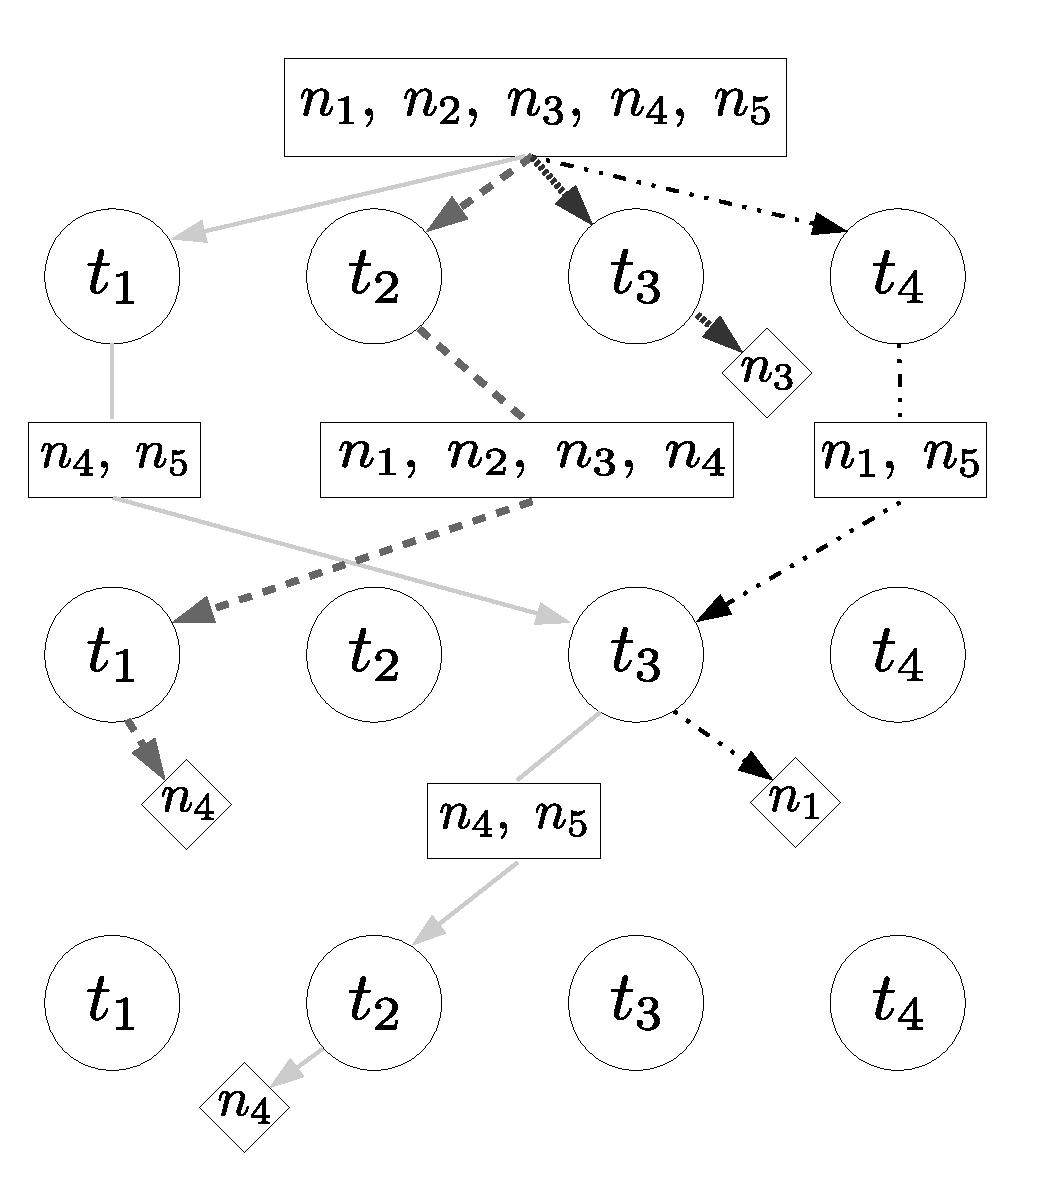
\includegraphics[height = 0.4\textheight]{figs/lex_graph.pdf}\label{fig:lex_graph}
  \caption{A graphical representation of 3 example parent selections using lexicase selection on the population in Table~\ref{tbl:ex}. The bold, dashed and dot-dashed lines indicate different selection paths through the test cases in circles. The boxes indicate the selection pool at each step in the process.}\label{fig:boxplot_eps_e}
\end{figure}

\paragraph{Complexity}
Can we analytically calculate the probability of selection an individual with less complexity than executing the lexicase selection algorithm? It appears not. Eqn.~\ref{eq:prob} has a worst-case complexity of $O(T^N)$ when all individuals are elite on $\mathcal{T}$, which discourages its use as a selection method. The lexicase selection algorithm samples the expected probabilities of each individual by recursing on random orders of cases in $\mathcal{T}$, considering one at a time rather than branching to consider all combinations of cases that could result in selection for each individual in question. This gives lexicase selection a complexity of $O(TN)$ for selecting a single parent, and therefore a complexity of $O(TN^2)$ per generation. 


 
\subsection{Effect of $N$ and $T$}
What does the an analysis of the probability of selection for lexicase selection tell us about how lexicase behaves for cases in which $|\mathcal{N}| << |\mathcal{T}|$?   $|\mathcal{T}| << |\mathcal{N}|$ ? 

The sampling of $P_{sel}$ done by lexicase is tied to the population size because lexicase selection conducts $N$ depth-first searches of the case orderings to choose $N$ parents. This implies that the value of $N$ determines the fidelity with which $P_{sel}$ is approximated via the sampling. Smaller populations will therefore produce poorer approximations of $P_{sel}$. 

The effectiveness of lexicase selection has also been tied to the number of fitness cases, $T$. When $T$ is small, there are very few ways in which individuals can be selected. For example, if $T$ = 2, an individual must be elite on one of these two cases to be selected. For continuous errors in which few individuals are elite, this means that only two individuals are likely to produce all of the children for the subsequent generation.

\subsection{Effect of different population structures}

\begin{enumerate}
\item compare probability of lexicase selection to probability of selection with tournament / roulette 
\item compare population structures: maintain correlation structure and vary population size/ number of test cases
\item see how many iterations of lexicase selection are required to converge on the probabilities of selection for the example problem in Table~\ref{tbl:ex}
\item population where there is one individual that sucks at everything but is good at other things - how does it compare to tournament selection probabilities?
\item do not assume that $N$ rounds of lexicase selection are conducted!
\end{enumerate}

\paragraph{Probabilities under tournament selection} We compare the probability of selection under lexicase selection to that using tournament selection with an indentical population and fitness structure. To do so we must first formulate the probability of selection for an individual undergoing tournament selection with $r$-size tournaments. Consider that the mean absolute error is used to aggregate the fitness cases. Then the fitness ranks of $\mathcal{N}$ can be calculated, with lower rank indicating better fitness. Let $S_i$ be the individuals in $\mathcal{N}$ with a fitness rank of $i$, and let $Q$ be the number of unique fitness ranks. Then Xie et. al.~\cite{xie_another_2007} showed that the probability of selecting an individual with rank $j$ in a single tournament is 
\begin{equation}
P_t = \frac{1}{|S_j|}\left( \left(\frac{\sum_{i=j}^Q{|S_i|}}{N}\right)^r - \left(\frac{\sum_{i=j+1}^Q{|S_i|}}{N}\right)^r \right)
\end{equation}

In Table~\ref{tbl:ex}, the selection probabilities for the example population are shown according to tournament selection. 

\section{Multi-objective Interpretation of Lexicase Selection}

Objectives and training cases are fundamentally different entities: objectives define the goals of the task being learned, whereas cases are the units by which progress towards those objectives is measured. By this criteria, lexicase selection and multi-objective optimization have historically been differentiated~\cite{helmuth_general_2015}, although there is clearly a ``multi-objective" interpretation of the behavior of lexicase selection with respect to the training cases. If we assume for a moment that we treat individual fitness cases as objectives to solve, we can consider most learning tasks to be high-dimensional many-objective optimization problems. At this scale, the most popular multi-objective methods (e.g. NSGA-II and SPEA-2) tend to perform poorly, a behavior that has been explained in literature~\cite{wagner_pareto-_2007, farina_optimal_2002}. Farina and Amato~\cite{farina_optimal_2002} point out two short-comings of these multi-objective methods when many objectives are considered: \begin{quote}
the Pareto definition of optimality in a multi-criteria decision making problem can be unsatisfactory due to essentially two reasons: the number of improved or equal objective values is not taken into account, the (normalized) size of improvements is not taken into account
\end{quote}

Lexicase selection is guarantees the return of individuals that are on the Pareto front with respect to the fitness cases. This is a necessary but not sufficient condition. In fact, lexicase selection only selects those individuals in the ``corners" of the Pareto front, meaning they are on the front {\it and} elite, globally, with respect to at least one fitness case. Put another way, no individual can be selected via lexicase selection unless it is elite with respect to at least one objective among the entire population, regardless of its performance on other objectives. 

Interestingly, the worst-case complexity of NSGA-II is the best-case complexity for lexicase selection. Add notes from discourse



\begin{figure}

\begin{minipage}{0.49\textwidth}
\centering
  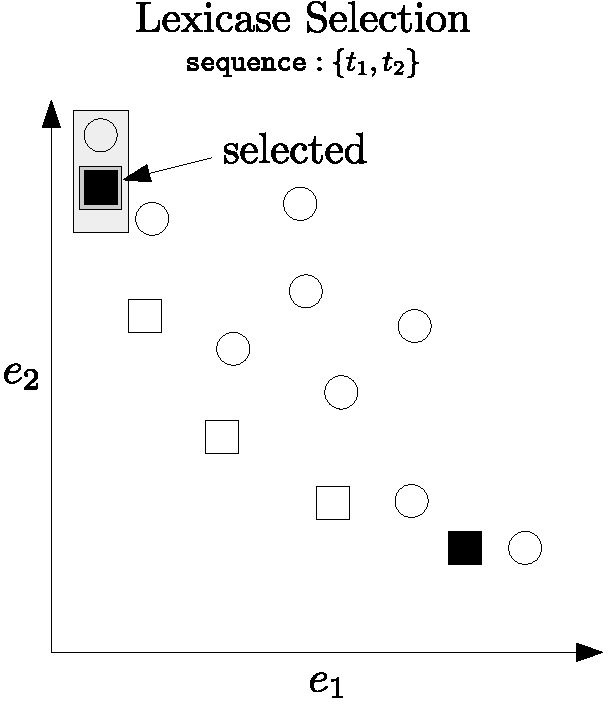
\includegraphics[width = \textwidth]{figs/lex_pareto.pdf}\label{fig:lex_pareto}
  \caption{An illustration of the performance of lexicase selection in a scenario involving two cases. Each point represents and individual in the population. The squares are individuals on the Pareto front. In each case, the selection ordering shown is $\{t_1,t_2\}$. }
\end{minipage}
\begin{minipage}{0.49\textwidth}
\centering
  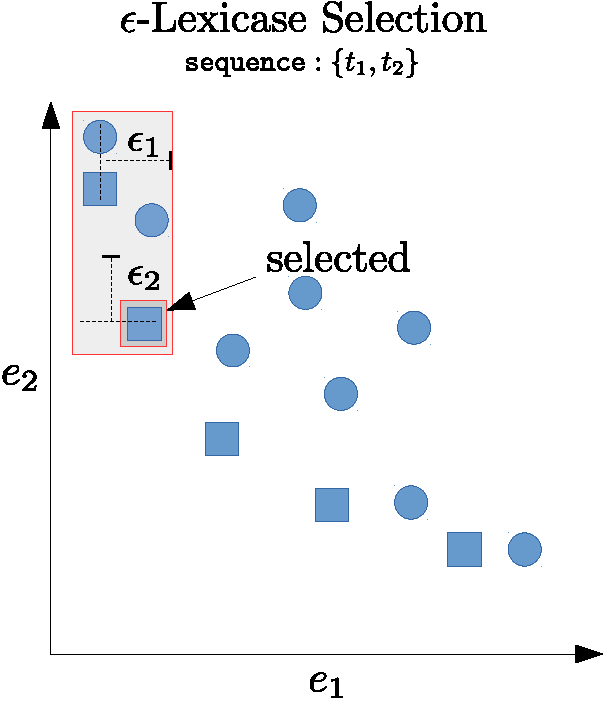
\includegraphics[width = \textwidth]{figs/ep-lex_pareto.pdf}\label{fig:ep-lex_pareto}
  \caption{An illustration of the performance of $\epsilon$-lexicase selection in a scenario involving two cases. Each point represents and individual in the population. The squares are individuals on the Pareto front. In each case, the selection ordering shown is $\{t_1,t_2\}$. }
\end{minipage}
\end{figure}

%Here is a detailed look at selection for program $n_1$:
%\begin{align*}
%P_{sel}(n_1 | \mathcal{N}, \mathcal{T}) &= \frac{1}{|\{t_1,t_2,t_3,t_4\}|}  \sum_{k_s \in \{t_2,t_4\}}{ P_{sel} \left( n_1 | \mathcal{N}(m|k_s \in K_m(\mathcal{T})), \mathcal{T}(t|t \neq k_s) \right)}  \\
%&= \frac{1}{4} \biggl[ P_{sel} \left( n_1 | \mathcal{N}(m|t_2 \in K_m(\mathcal{T})), \mathcal{T}(t|t \neq t_2) \right) + P_{sel} \left( n | \mathcal{N}(m|t_4 \in K_m(\mathcal{T})), \mathcal{T}(t|t \neq t_4) \right) \biggl] \\
%&= \frac{1}{4} \left[ P_{sel} ( n | \{n_1, n_2, n_3, n_4\}, \{t_1, t_3, t_4\} ) + P_{sel} ( n | \{n_1, n_5 \} , \{t_1, t_2, t_3\} ) \biggl] \\
%&= \frac{1}{4} \biggl[ \frac{1}{|\{t_1, t_3, t_4\}} \sum_{k_s \in \{t_4\}}{ P_{sel} \left( n | \mathcal{N}(m|k_s \in K_m(\mathcal{T}(t|t \neq t_2)), \mathcal{T}(t|t \notin \{t_2,k_s\}) \right)} \\
%& + \frac{1}{|\{t_1, t_2, t_3\}|} \sum_{k_s \in \{t_2,t_3\}}{ P_{sel} \left( n | \mathcal{N}(m|k_s \in K_m(\mathcal{T}(t|t \neq t_2)), \mathcal{T}(t|t \notin \{t_4,k_s\}) \right)}\biggl] \\
%&= \frac{1}{4} \biggl[ \frac{1}{3} P_{sel} ( n_1 | \{n_1\}, \{t_1, t_3\})  + \frac{1}{3} \biggl( P_{sel} ( n_1 | \{n_1\}, \{t_1,t_3\} ) \\
%&+ P_{sel} ( n_1 | \{n_1\}, \{t_1,t_2\} ) \biggl) \biggl]\\
%&= \frac{1}{4} \biggl[ \frac{1}{3}(1) + \frac{1}{3}(1 + 1) \biggl]\\
%&= \frac{1}{4} 
%\end{align*}
Here we define Pareto dominance relations with respect to the training cases. 

\medskip
\noindent {\bf Definition 1:} $n_1$ {\it dominates} $n_2$, i.e., ${n_1} \prec {n_2}$, if $e_j(n_1) \leq e_j(n_2) \;
\forall j  \in \{1,\dots,T\}$ and $\exists j \in \{1,\dots,T\}$ for which $e_j(n_1) < e_j(n_2)$. \bigskip
\bigskip

\medskip
\noindent {\bf Definition 2:} The {\it Pareto set} of $\mathcal{N}$ is the subset of $\mathcal{N}$ that is non-dominated with respect to $\mathcal{N}$; i.e., $n \in \mathcal{N}$ is in the Pareto set if $n \nprec m \; \forall \; m \in \mathcal{N}$. 
\bigskip

\medskip
\noindent {\bf Definition 3:} $n \in \mathcal{N}$ is a {\it Pareto set boundary} if $n$ is in the Pareto set of $\mathcal{N}$ and $\exists j \in \{1,\dots,T\}$ for which $e_j(n_1) \leq e_j(m) \; \forall \; m \in \mathcal{N}$. \bigskip
\bigskip

With these definitions in mind, we show that individuals selected by lexicase are on the Pareto set boundaries. 

\medskip
\noindent \textbf{Theorem 1:} If individuals from a population $\mathcal{N}$ are selected by lexicase selection, those individuals are Pareto set boundaries of $\mathcal{N}$ with respect to $\mathcal{T}$. 
\medskip

\noindent \textbf{Proof:} First, we prove (by supposing a contradiction) that individuals selected by lexicase are in the Pareto set. Second, we prove these individuals to be Pareto set boundaries. 

First: Let $n_1, n_2 \in \mathcal{N}$ be individuals in a population selected by lexicase selection. Suppose $n_1 \prec n_2$. Then $e_j(n_1) \leq e_j(n_2) \;
\forall j  \in \{1,\dots,N\}$ and $\exists j \in \{1,\dots,T\}$ for which $e_j(n_1) < e_j(n_2)$. Therefore $n_1$ is selected for every case that $n_2$ is selected, and $\exists t \in \mathcal{T}$ for which $n_2$ is removed from selection due to $n_1$. Hence, $n_2$ cannot be selected by lexicase selection and the supposition is false. Therefore $n_1$ and $n_2$ must be in the Pareto set. 

Second: let $n$ be an individual selected from population  $\mathcal{N}$ by lexicase selection. Then by definition of the Algorithm 1, $\exists j \in \{1,\dots,T\}$ for which $e_j(n) \leq e_j(m) \; \forall \; m \in \mathcal{N}$. Therefore, since $n$ is in the Pareto set of $\mathcal{N}$ and according to Definition 3, $n$ is a Pareto set boundary of $\mathcal{N}$.  
\bigskip



\paragraph{Extension to $\epsilon$-lexicase selection}
We can extend our multi-objective analysis to $\epsilon$-lexicase selection for conditions in which $\epsilon$ is pre-defined for each fitness case, i.e. in static and dynamic cases, but not when $\epsilon$ is recalculated for each selection pool. We first define $\epsilon$ elitism in terms of a relaxed dominance relation and a relaxed Pareto set. We define the dominance relation with respect to $\epsilon$ as follows:


\medskip
\noindent {\bf Definition 4:} $n_1$ {\it $\epsilon$-dominates} $n_2$, i.e., ${n_1} \prec_{\epsilon} {n_2}$, if $e_j(n_1) + \epsilon_j \leq e_j(n_2)  \;
\forall j  \in \{1,\dots,T\}$ and $\exists j \in \{1,\dots,T\}$ for which $e_j(n_1) + \epsilon_j < e_j(n_2) $, where $\epsilon_j>0$ is defined according to Eqn.~\ref{eq:ep}\bigskip
\bigskip
\medskip

\noindent {\bf Definition 5:} The {\it $\epsilon$-Pareto set} of $\mathcal{N}$ is the subset of $\mathcal{N}$ that is non-$\epsilon$-dominated with respect to $\mathcal{N}$; i.e., $n \in \mathcal{N}$ is in the Pareto set if $n \nprec_{\epsilon} m \; \forall \; m \in \mathcal{N}$. 
\bigskip

\medskip
\noindent {\bf Definition 6:} $n \in \mathcal{N}$ is an {\it $\epsilon$-Pareto set boundary} if $n$ is in the $\epsilon$-Pareto set of $\mathcal{N}$ and $\exists j \in \{1,\dots,T\}$ for which $e_j(n_1) + \epsilon_j \leq e_j(m) \; \forall \; m \in \mathcal{N}$, where $\epsilon_j$ is defined according to Eqn~\ref{eq:ep}. \bigskip


\medskip
\noindent \textbf{Theorem 2:} If $\epsilon$ is defined according to Eqn.~\ref{eq:ep}, and if individuals are selected from a population $\mathcal{N}$ by $\epsilon$-lexicase selection, then those individuals are elements are $\epsilon$-Pareto set boundaries of $\mathcal{N}$.  
\medskip


\noindent \textbf{Proof:} First: Let $n_1, n_2 \in \mathcal{N}$ be individuals in a population selected by $\epsilon$-lexicase selection. Suppose $n_1 \prec_{\epsilon} n_2$. Then $n_1$ is selected for every case that $n_2$ is selected, and $\exists t \in \mathcal{T}$ in every selection event for which $n_2$ is removed from selection due to $n_1$. Hence, $n_2$ cannot be selected by lexicase selection and the supposition is false, and therefore $n_1$ and $n_2$ must be in the Pareto set of $\mathcal{N}$. 

Second: let $n$ be an individual selected from population $\mathcal{N}$ by static or semi-dynamic $\epsilon$-lexicase selection. Then by definition of Algorithm 2 or 3, $\exists j \in \{1,\dots,T\}$ for which $e_j(n) \leq e_j(m) \; \forall \; m \in \mathcal{N}$. Therefore, since $n$ is in the $\epsilon$-Pareto set of $\mathcal{N}$ and according to Definition 3, $n$ is an $\epsilon$-Pareto set boundary of $\mathcal{N}$.  
\bigskip

The notion of the selection of Pareto set boundaries by lexicase selection is illustrated in Figure~\ref{fig:lex_pareto} for a scenario with two fitness cases. Given the case sequence $\{t_1, t_2\}$, individuals would first be filtered to the two elite individuals on $e_1$, and then to the individual among those two that is best on $e_2$, i.e. the selected square individual. Note that this individual exists at the Pareto set boundary. Given the opposite order of cases, i.e. $\{t_2, t_1\}$, the individual on the other end of the Pareto set (the other boundary in case space) would be selected.   

Consider the analogous case for semi-dynamic $\epsilon$-lexicase selection illustrated in Figure~\ref{fig:ep-lex_pareto}. 

\section{Illustrative Example}
\paragraph{Example}
As an example of calculating absolute probabilities, we consider the illustrative problem from the original lexicase selection paper~\cite{spector_assessment_2013}, shown in Table~\ref{tbl:ex}. Using Eqn.~\ref{eq:prob}, the probabilities for each individual can be calculated as follows:

\begin{align*}
P_{sel}(n_1) &=& 1/4*(1/3*(1)+1/3*(1+1)) = 0.25 \\
P_{sel}(n_2) &=& 1/4*(0) = 0 \\
P_{sel}(n_3) &=&1/4*(1/3*(1+1/2*(1))+1/3*(1)) = 0.20833 \\
P_{sel}(n_4) &=& 1/4*(1/3*(1/2*(1)+1)+1/3*(1)) = 0.20833 
\end{align*}

\begin{table}
\centering
\caption{Example population from original lexicase paper (Spector 2013).}\label{tbl:ex}
\begin{tabular}{l|cccc|c|r|rr}
Program & \multicolumn{4}{c}{Test} & $\mathcal{K}(\mathcal{T})$ & MAE & $P_{sel}$ & $P_{t}$\\
& $t_1$ & $t_2$ & $t_3$ & $t_4$ & \\ \hline
$n_1$ & 2 & 2 & 4 & 2 & $\{t_2,t_4\}$ &	2.5		&	0.25 	& 	0.28	\\
$n_2$ & 1 & 2 & 4 & 3 & $\{t_2\}$		&	2.5		&	0.00	&	0.28	\\
$n_3$ & 2 & 2 & 3 & 4 & $\{t_2,t_3\}$ &	2.75	& 	0.33	&	0.12	\\
$n_4$ & 0 & 2 & 5 & 5 & $\{t_1,t_2\}$ &	3.0		& 	0.208	&	0.04	\\
$n_5$ & 0 & 3 & 5 & 2 & $\{t_1,t_4\}$ &	2.5		&	0.208	&	0.28
\end{tabular}
\end{table}

\begin{table}
\centering
\scriptsize
\caption{Example population with test case performances and selection probabilities according to the different algorithms.}\label{tbl:ex2}
\begin{tabularx}{\textwidth}{X|rrrrr|r|R{2em}R{2em}R{2em}R{2em}R{2em}}\toprule
$\mathcal{N}$ & \multicolumn{5}{c}{Cases} & Mean & \multicolumn{5}{c}{Probability of Selection} \\
& $t_1$ & $t_2$ & $t_3$ & $t_4$ & $t_5$ &&	tourn	&	lex	&	$\epsilon$ lex static	&	$\epsilon$ lex semi	&	$\epsilon$ lex dyn\\ \midrule
$n_1$	&0.0	&	1.1	&	2.2	&	3.0	&	5.0 & 2.26	&	0.111	&	0.200	&	0.000	&	0.067	&	0.033\\ 
$n_2$	&0.1	&	1.2	&	2.0	&	2.0	&	6.0 & 2.26	&	0.111	&	0.000	&	0.150	&	0.117	&	0.200\\ 
$n_3$	&0.2	&	1.0	&	2.1	&	1.0	&	7.0 & 2.26	&	0.111	&	0.000	&	0.150	&	0.117	&	0.117\\ 
$n_4$	&1.0	&	2.1	&	0.2	&	0.0	&	8.0 & 2.26	&	0.111	&	0.200	&	0.300	&	0.200	&	0.167\\ 
$n_5$	&1.1	&	2.2	&	0.0	&	4.0	&	4.0 & 2.26	&	0.111	&	0.200	&	0.000	&	0.050	&	0.050\\ 
$n_6$	&1.2	&	2.0	&	0.1	&	5.0	&	3.0 & 2.26	&	0.111	&	0.000	&	0.000	&	0.050	&	0.033\\ 
$n_7$	&2.0	&	0.1	&	1.2	&	6.0	&	2.0 & 2.26	&	0.111	&	0.000	&	0.133	&	0.133	&	0.133\\ 
$n_8$	&2.1	&	0.2	&	1.0	&	7.0	&	1.0 & 2.26	&	0.111	&	0.000	&	0.133	&	0.133	&	0.217\\ 
$n_9$	&2.2	&	0.0	&	1.1	&	8.0	&	0.0 & 2.26	&	0.111	&	0.400	&	0.133	&	0.133	&	0.050\\  \midrule
$\epsilon$	&	0.9	& 0.9	&	0.9	&	2.0	& 2.0	&&&&&&\\ \bottomrule
\end{tabularx}
\end{table}

\paragraph{Illlustrative Example 2} A more complex population semantic structure is presented in Table~\ref{tbl:ex2} featuring floating point errors. In this case, the population semantics are completely unique, although they result in the same mean error across the training cases, as shown in the ``Mean" column. As a result, tournament selection picks uniformly from among these individuals. 

As mentioned earlier, with unique populations, lexicase selection is proportional to the number of cases for which an individual is elite. This leads lexicase selection to pick from among the 4 individuals that are elite on cases, i.e. $n_1$ ($t_1$), $n_4$ ($t_4$), $n_5$ ($t3$), and $n_9$ ($t_2$,$t_5$), with respective probabilities 0.2, 0.2, 0.2, and 0.4. 

Due to its strict definition of elitism, lexicase selection does not account for the fact other individuals are very close to being elite on these cases as well. The $\epsilon$-lexicase variants address this as noted by the smoother distribution of selection probabilities among this population. Focusing first on static $\epsilon$-lexicase selection, it is worth illustrating the pass conditions for the population by applying the $\epsilon$ threshold, yielding the following semantics:

\begin{center}
\begin{tabular}{lrrrrr}
& $t_1$ & $t_2$ & $t_3$ & $t_4$ & $t_5$ \\
$n_1$	&0	&	1	&	1	&	1	&	1\\ 
$n_2$	&0	&	1	&	1	&	0	&	1\\ 
$n_3$	&0	&	1	&	1	&	0	&	1\\ 
$n_4$	&1	&	1	&	0	&	0	&	1\\ 
$n_5$	&1	&	1	&	0	&	1	&	1\\ 
$n_6$	&1	&	1	&	0	&	1	&	1\\ 
$n_7$	&1	&	0	&	1	&	1	&	0\\ 
$n_8$	&1	&	0	&	1	&	1	&	0\\ 
$n_9$	&1	&	0	&	1	&	1	&	0\\ 
\end{tabular}
\end{center}
 
The selection probabilities for static $\epsilon$ lexicase selection are equivalent to the selection probabilities of lexicase selection on this converted semantic matrix. Despite elitism on case $t_1$, $n_1$ is not selected since $n_2$ and $n_3$ are $\epsilon$-elite on this case as well as $t_4$. Consider $n_4$, which has a higher probability of selection under static $\epsilon$-lex than lexicase selection. This is due to it being $\epsilon$-elite on a unique combination of cases: $t_3$ and $t_4$. Lastly $n_8$ is selected in equal proportions to $n_7$ and $n_6$ since all are within $\epsilon$ of the elite error on the same cases. 

Semi-dynamic $\epsilon$ lexicase selection allows for all 9 individuals to be selected with varying proportions that are similar to those derived for static $\epsilon$ lexicase selection. Selection probabilities for $n_1$ illustrate the differences in the static and semi-dynamic variants: $n_1$ has a chance for selection in the semi-dynamic case because when $t_1$ is selected as the first case, $n_1$ is within $\epsilon$ of the best case errors {\it among the pool}, i.e. $\{n_1$, $n_2$, $n_3\}$, for any subsequent order of cases. The probability of selection for $n_5$ and $n_6$ follow the same pattern.

Dynamic $\epsilon$-lexicase selection produces the most differentiated selection pressure for this example. Consider individual $n_8$ which is the most likely to be selected for this example. It is selected more often than $n_7$ or $n_9$ due to the adaptations to $\epsilon$ as the selection pool is winnowed. For example, $n_8$ is selected by case sequence $\{t_2,t_1,t_3\}$, for which the selection pool takes the following form after each case: $\{n_7, n_8, n_9\}, \{n_7, n_8\}, \{n_8\}$. Under the other semi-dynamic $\epsilon$ lexicase selection, $n_7$ and $n_8$ would not be removed by these cases due to the fixed nature of $\epsilon$ for those cases. The probabilities of selection for the population in Table~\ref{tbl:ex2} is shown graphically in Figure~\ref{fig:prob}. 

\begin{figure}
\centering
  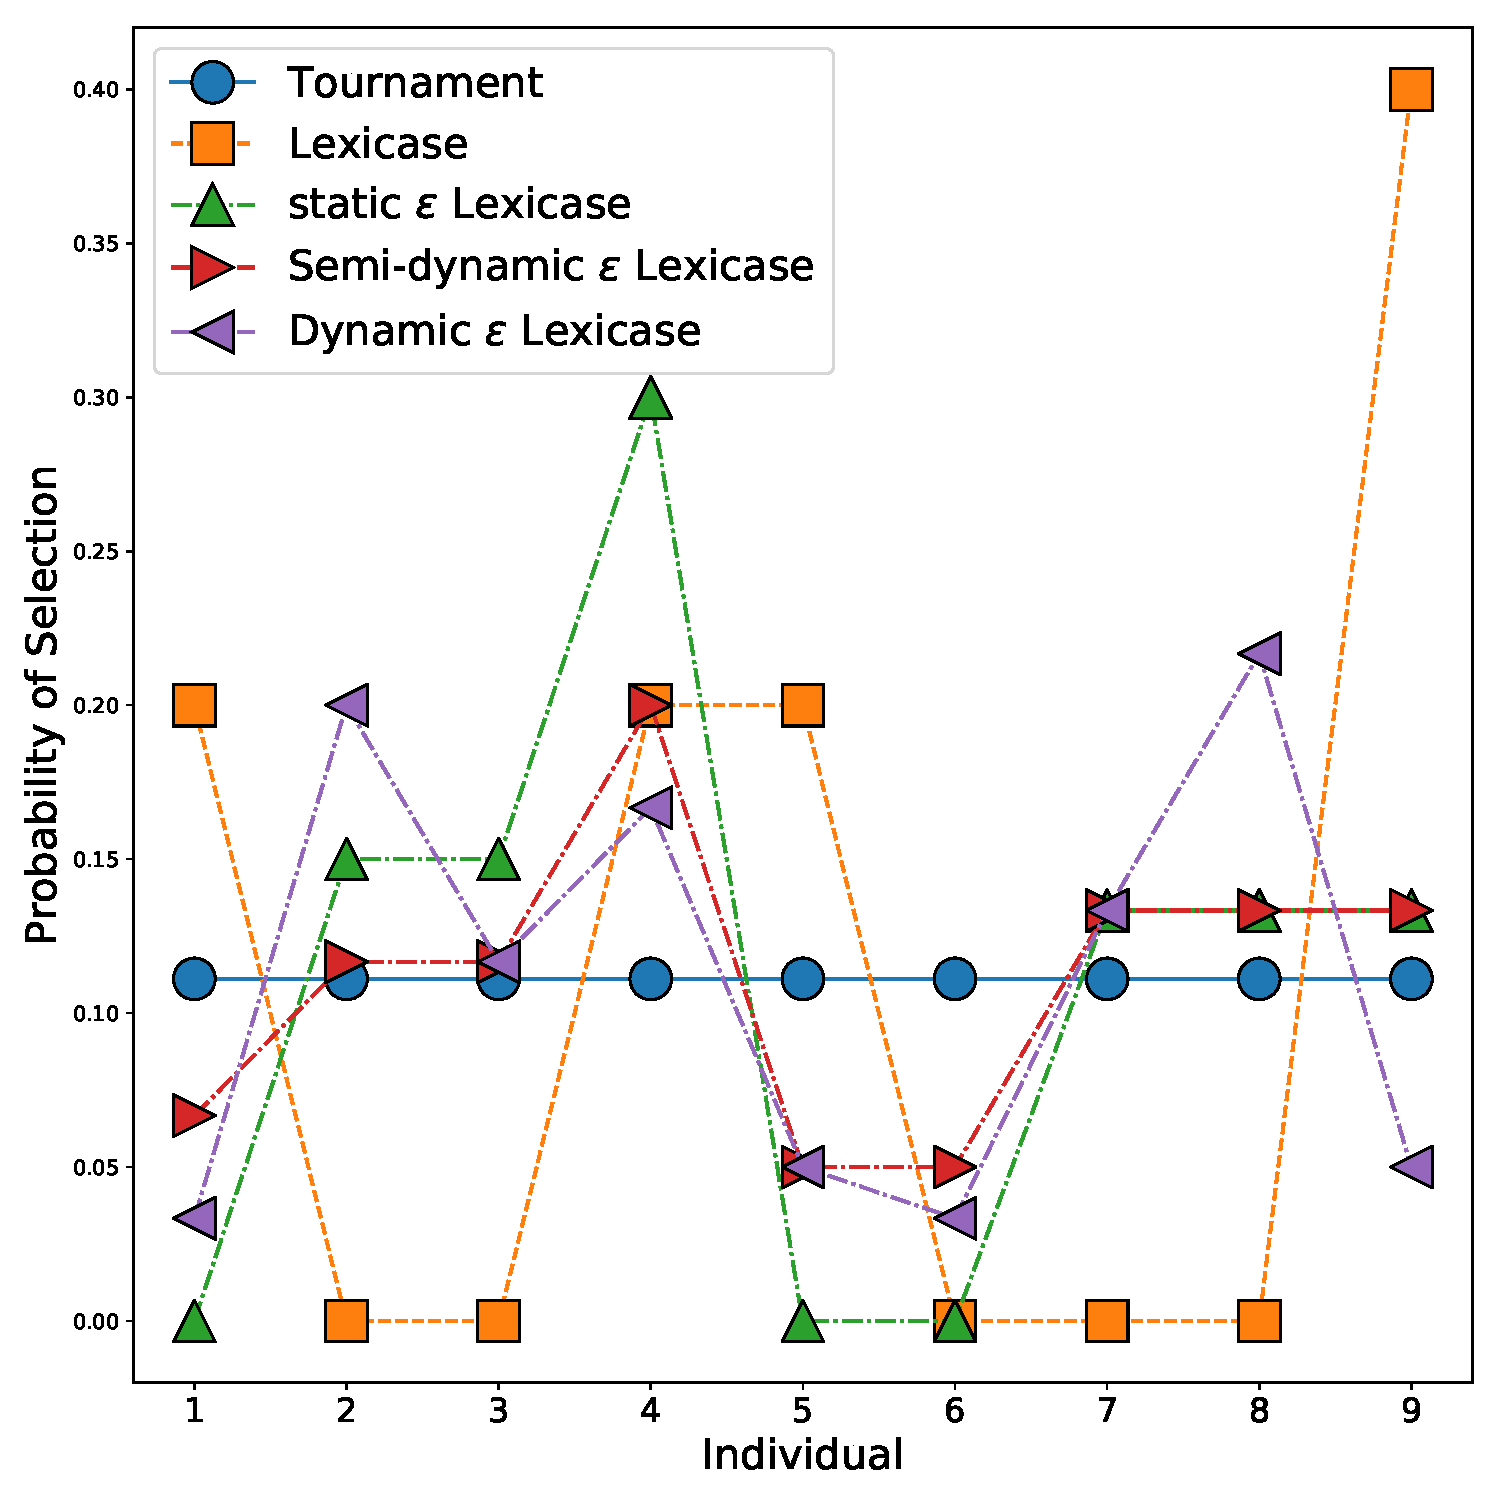
\includegraphics[height = 0.4\textheight]{figs/probabilities.pdf}\label{fig:prob}
  \caption{A graphical representation of the probabilities of selection for the population in Table~\ref{tbl:ex2} according to different selection methods.}\label{fig:boxplot_eps_e}
\end{figure}

 
\section{Related Work}\label{s:3}


\section{Experimental Analysis} \label{s:4}

\begin{table}
\scriptsize
\caption{GP settings.}\label{tbl:symreg_settings}
\begin{tabularx}{\columnwidth}{X R{0.57\columnwidth}} \toprule
Setting& Value \\ \midrule
Population size & 1000 \\
Crossover / mutation & 60/40\% \\
Program length limits & [3, 50] \\ 
ERC range & [-1,1] \\
Generation limit & 1000 \\
Trials & 50 \\
Terminal Set & \{$\mathbf{x}$, ERC, $+$, $-$, $*$, $/$, $\sin$, $\cos$, $\exp$, $\log$\}\\
Elitism & keep best \\
\end{tabularx}
\end{table}
\begin{table}
\scriptsize
\caption{Regresion problems used for method comparisons.}\label{tbl:regression}
\begin{tabularx}{\columnwidth}{X r r } \toprule
Problem & Dimension & Samples \\ \midrule
Airfoil & 5	& 1503 \\
Concrete	& 	8	& 1030	\\
Crime	&	127	&	1993	\\
ENC & 8 & 768 \\
ENH & 8 & 768 \\
Housing & 14 & 506 \\
Tower & 25 & 3135 \\
UBall5D & 5 & 6024 \\ 
Yacht	& 6	&	309	\\ \midrule
\end{tabularx}
\end{table}
\begin{table}
\scriptsize
\caption{Dynamical systems used for method comparisons. The systems were simulated four times using initial conditions within stable basins of attraction. $\gamma$ indicates zero-mean, unit-variance Gaussian noise. }\label{tbl:ode}
\rowcolors{4}{white}{LightCyan}
\begin{tabularx}{\columnwidth}{L{0.25\columnwidth} L{0.3\columnwidth} L{0.19\columnwidth}  R{0.1\columnwidth}} 
Problem & Equations & Initial Conditions	& Samples \\ \midrule
Bacterial Respiration & $\dot{x} = 20 - x - \frac{x \cdot y}{1+0.5 \cdot x^2}$ , $ \dot{y} = 10 - \frac{x \cdot y}{1+0.5 \cdot x^2}$	& $x_0=5 \pm \gamma$, $y_0=10 \pm 0.1\gamma$ & 400 \\
Bar Magnets & $\dot{\theta} = 0.5 \cdot \sin (\theta - \phi) - \sin (\theta)$,  $ \dot{\phi} = 0.5 \cdot \sin (\phi - \theta) - \sin (\phi)$	&  $\theta_0 \in [-2\pi,2\pi]$, $\phi_0 \in [-2\pi,2\pi]$ & 400 \\
Glider & $\dot{v} = - 0.05 \cdot  v^2 - sin (\theta)$	, $ \dot{\theta} = v - \cos (\theta)/v$	& $v_0=5 \pm \gamma$, $\theta_0=10 \pm 0.1\gamma$ & 400 \\
Lotka-Volterra interspecies dynamics & $\dot{x} = 3  \cdot x - 2  \cdot x \cdot y - x^2$, $ \dot{y} = 2 \cdot y - x \cdot y - y^2$	&  $x_0=[1,4,8,3]$, $y_0 = [3, 1, 2, 3]$ & 400 \\
Predator Prey & $\dot{x} = x  \cdot \left( 4 - x - \frac{y}{1+x} \right)$, $ \dot{y} = 2 \cdot y - x \cdot y - y^2$ 	& $x_0=5 \pm \gamma$, $y_0=10 \pm 0.1\gamma$  & 400 \\
Shear Flow & $\dot{\theta} = \cot (\phi) \cdot cos(\theta)$, $ \dot{\phi} = \left(\cos ^2 (\phi) + 0.1 \cdot  \sin^2 (\phi)\right) \cdot sin(\theta)$	&  $\theta_0 \in [-\pi,\pi]$, $\phi_0 \in [-\pi/2,\pi/2]$ & 400 \\
van der Pol oscillator & $\dot{x} = 10 \cdot  \left(y - \frac{1}{3} \cdot (x^3-x) \right)$	, $ \dot{y} = -\frac{1}{10} \cdot x$		& $x,y \in [0,1]$  & 400 \\ \midrule
\end{tabularx}
\end{table}
\begin{table}
\begin{tabularx}{\columnwidth}{X X r r r} 
\multicolumn{5}{c}{Program Synthesis}\\ 
Problem	& Input & Output	& Training Cases & Test Cases \\\midrule
Number IO & integer in [-100,100], float in [-100.0, 100.0]	&	printed float & 25 & 1000 \\
Wallis PI & integer in [1, 200] & float &	150 & 50 \\
Vector Average & vector of float of length [1,50] with each float in [-1000.0, 1000.0]	& float &	100	&	1000 \\ 
\bottomrule
\end{tabularx}
\end{table}

\subsection{Effect of population structure on probabilities of selection}


\subsection{Results}\label{s:4 results}
\begin{figure}
\centering
  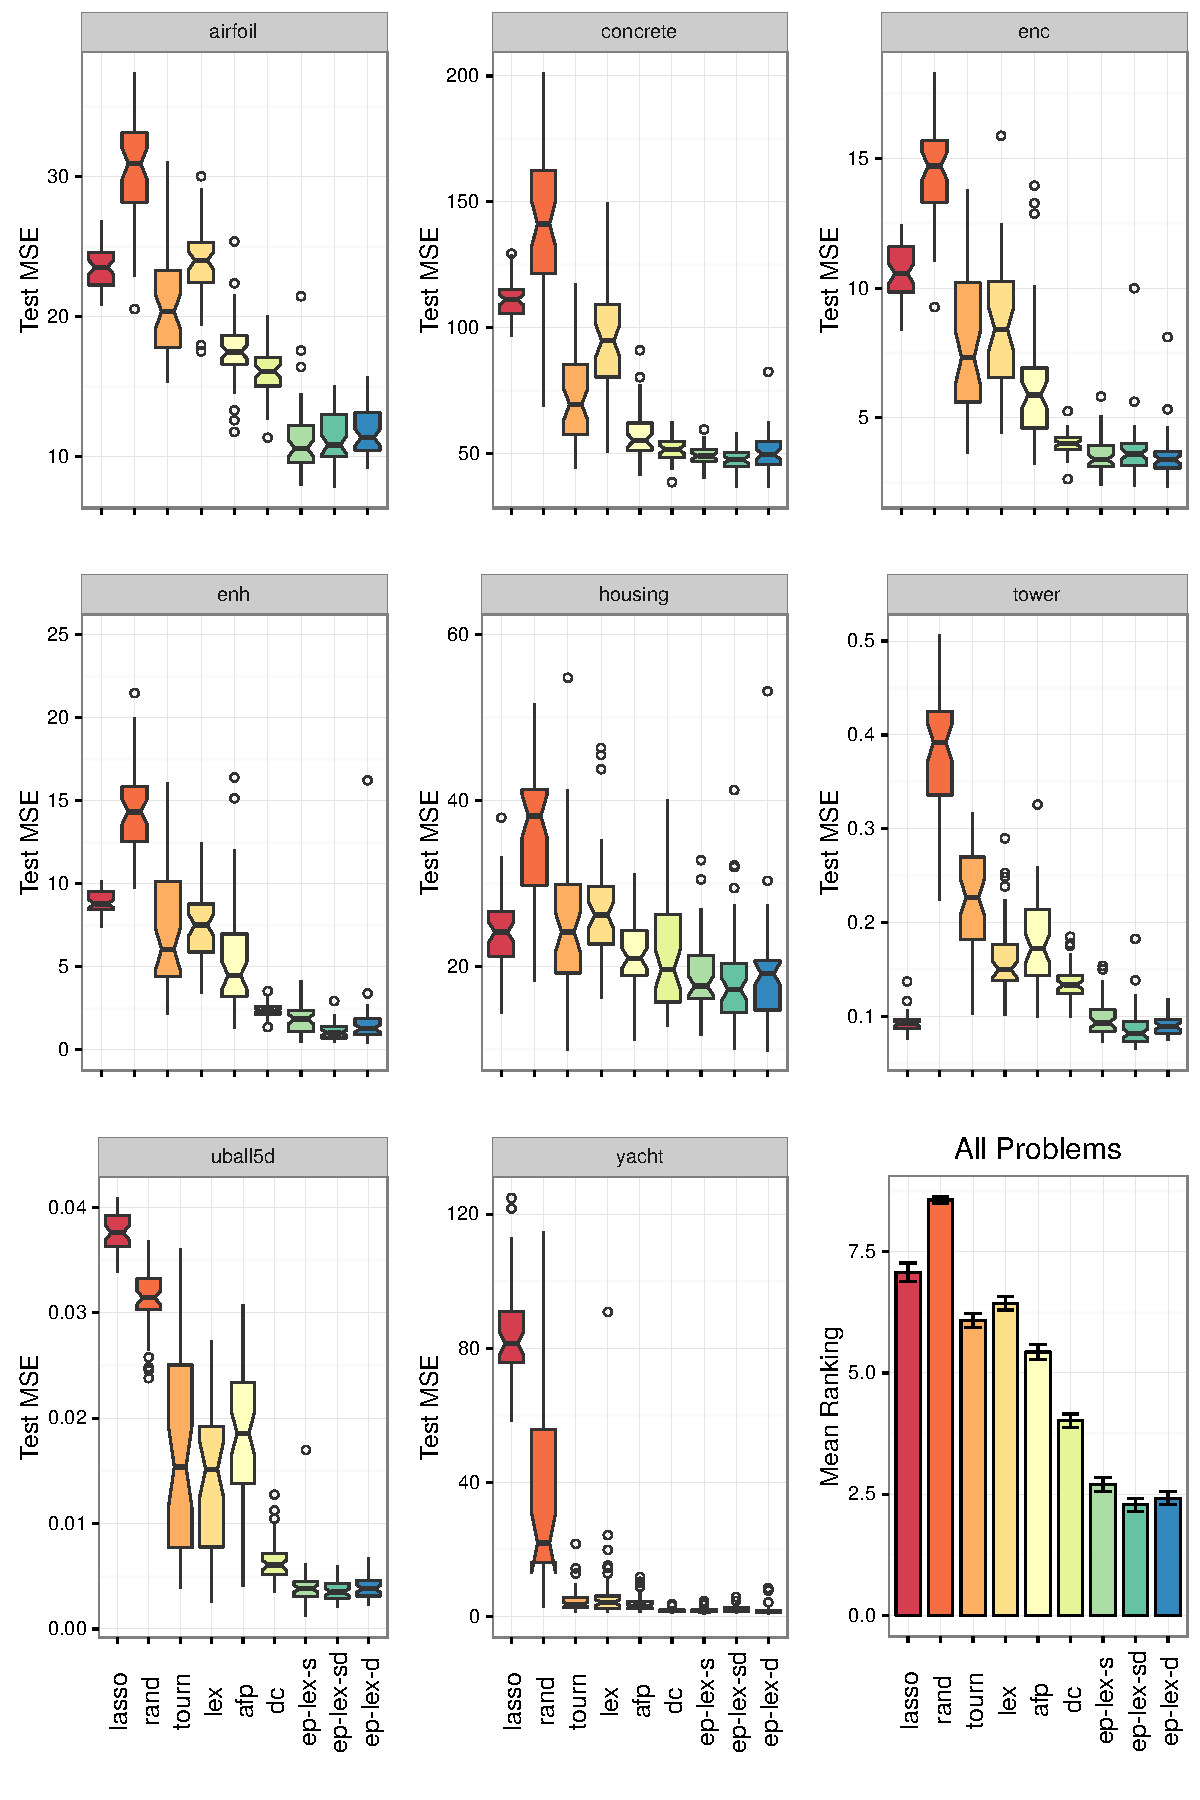
\includegraphics[width=\textwidth]{figs/regression_boxplots.pdf}\\
  \caption{Boxplots of the mean squared error on the test set for 50 randomized trials of each algorithm on the regression benchmark datasets.}\label{fig:boxplot_reg}
\end{figure}

\begin{figure}
\centering
  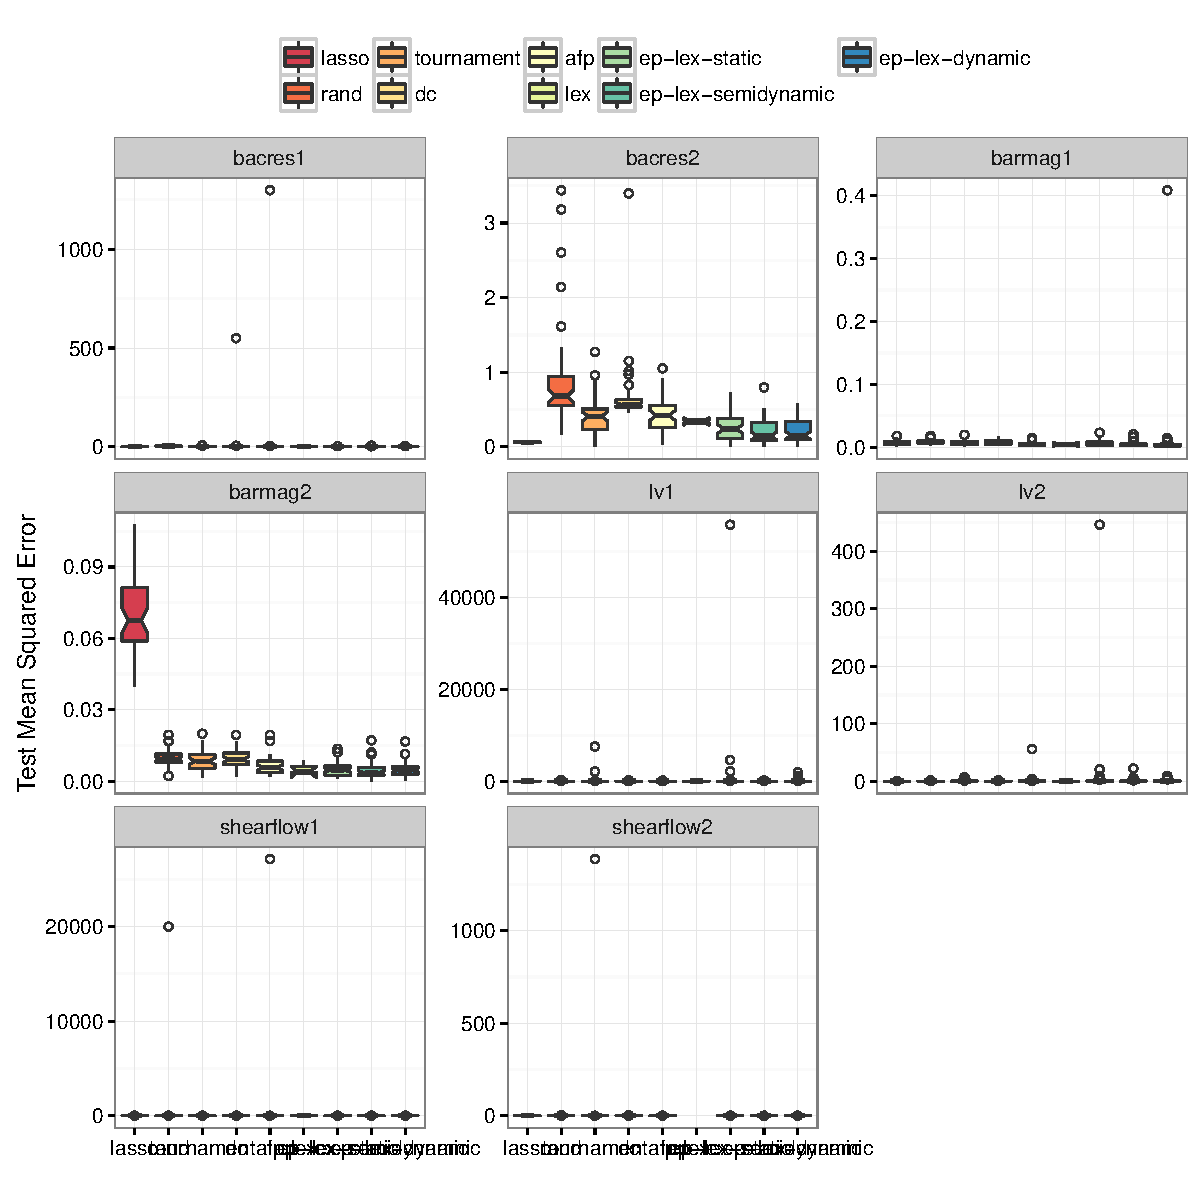
\includegraphics[width=\textwidth]{figs/ode_boxplots.pdf}\\
  \caption{Boxplots of the mean squared error on the test set for 50 randomized trials of each algorithm on the regression benchmark datasets.}\label{fig:boxplot_reg}
\end{figure}

\section{Discussion}\label{s:5}


\section{Conclusions}\label{s:6}

\section{Acknowledgments}



\bibliographystyle{abbrv}
\bibliography{epsilon_lexicase}


\end{document}
